\documentclass[pdf]{beamer}
\mode<presentation>{} 

\usepackage{hyperref}
\usepackage{pgf}
\usepackage{tikz}
\usetikzlibrary{trees}
\usetikzlibrary{arrows,automata}
\usetikzlibrary{automata,positioning}
\usetikzlibrary{shapes}
\usepackage{tikz-qtree,tikz-qtree-compat}
\usepackage{mathtools,enumerate,amssymb}
\usepackage[utf8]{inputenc}
\usepackage[T1]{fontenc}
\usepackage{graphicx}
\usepackage{tabularx}

\title{Introducere în Securitatea informatică}
\subtitle{Securitate informatică}
\AtBeginSection[]{}

\setbeamertemplate{sidebar right}{}
\setbeamertemplate{footline}{%
\hfill\usebeamertemplate***{navigation symbols}
\hspace{1cm}\insertframenumber{}/\inserttotalframenumber}

\begin{document}

\begin{frame}
	\titlepage
	
\begin{flushright}
Mihai-Lica Pura\\
\end{flushright}

\end{frame}



\begin{frame}{Cuprins}
\begin{itemize}
\item
Nevoia de securitate informatică/Motivație
\item
Security services and mechanisms
\item
CIA triad
\item
Definiție
\item
Vulnerabilități
\item
Amenințări
\item
Riscuri de securitate
\item
Atacuri cibernetice
\item
Rapoarte privind securitatea informatică
\item
Niveluri de securitate
\item
Curricula în Securitatea informației
\item
Information Security Standards and Best Practices
\item
Bibliografie
\end{itemize}
\end{frame}



\begin{frame}{Nevoia de securitate informatică/Motivație}
\begin{itemize}
\item
Carduri bancare
\begin{itemize}
\item
operații la bancomat
\item
plăți prin POS
\item
plăți electronice prin Internet
\end{itemize}
\item
Internet banking/Mobile banking
\item
Email account and other accounts
\item
acces WiFi
\item
ANAF - depunere declații fiscale (persoane fizice și juridice)

\url{https://static.anaf.ro/static/10/Anaf/Declaratii_R/instructiuni/etape_depunere.htm}

\url{https://static.anaf.ro/static/10/Anaf/Declaratii_R/instructiuni/Instructiuni_D200.htm}

\end{itemize}
\end{frame}



\begin{frame}{Nevoia de securitate informatică/Motivație}
\begin{itemize}
\item
CNAS - raportări pentru furnizorii de servicii medicale, medicamente și dispozitive medicale

\url{http://www.cnas.ro/casmb/page/procedura-de-inregistrare-a-certificatelor-digitale.html}

\item
MySMIS 2014 - Access EU funds – Ministry of European Funds

\url{https://2014.mysmis.ro/}

\url{http://www.fonduri-ue.ro/mysmis}

\item
SEAP - Sistemul Electronic de Achiziții Publice

\url{http://licitatiiseap.ro/seap/}

\url{https://www.e-licitatie.ro/}

\item
Centrul Național de Administrare a Registrelor Naționale Notariale - Infonot

\url{https://www.infonot.eu/}

\item
etc.

\end{itemize}
\end{frame}



\begin{frame}{Nevoia de securitate informatică/Motivație}
\begin{itemize}
\item
"Information is an asset which, like other important business assets, has value to an organization and consequently needs to be suitable protected." (ISO 27002:2005)

\item
"Whatever form the information takes, or means by which it is shared or stored, it should always be appropriately protected." (ISO 27002:2005)

\item
Informația este un bun valoros atât pentru persoanele fizice, cât și pentru organizații, și trebuie să fie protejată.
\end{itemize}
\end{frame}



\begin{frame}{Security services and security mechanisms}
\begin{itemize}
\item
Open Systems Security Architecture (X.800)
\begin{itemize}
\item
the first stage in the development of 
a suite of standards to support security services and mechanisms
\item 
general description of security services and the related mechanisms that can be used to provide these services
\item
Security services:
\begin{itemize}
\item
Authentication;
\item
Access Control;
\item
Data Confidentiality;
\item
Data Integrity;
\item
Non-Repudiation.
\end{itemize}
\end{itemize}

\end{itemize}
\end{frame}



\begin{frame}{Security services}
\begin{itemize}
\item
ISO 7498-2 (1989) and X.800:
\begin{itemize}
\item
\textbf{Identification and authentication} - the ability to identify and uniquely authenticate all users of a system
\item
\textbf{Authorisation/access control} - the ability to allow or prohibit users from accessing the information assets of an organisation
\item
\textbf{Confidentiality} - the ability to ensure that information assets are only available to those who are authorised to access them
\item
\textbf{Integrity} - the ability to ensure that information is complete and uncorrupted and that it has not been altered in any way
\item
\textbf{Non-repudiation/non-denial} - the ability to ensure that users do not deny their actions
\end{itemize}
\end{itemize}
\end{frame}



\begin{frame}{Security services}
\begin{itemize}
\item
ITU-T Recommendations Report X.805 in support of the X.800 and ISO 7498-2 (1989) 
\item
adds 3 new dimensions:
\begin{itemize}
\item
Privacy
\item
Availability
\item
Communication Security
\end{itemize}
\end{itemize}
\end{frame}



\begin{frame}{Security services}
\begin{itemize}
\item
\textbf{Authentication} - serves to confirm the identities of the communicating entities
\begin{itemize}
\item
the recipient of the message should be sure that the  message came from the source that it claims to be
\item
all communicating parties should be sure that the connection is not interfered with by unauthorized party
\end{itemize}
\item
\textbf{Access Control} - protects against unauthorised use of network resources
\begin{itemize}
\item
who can have access to a resource
\item
under what conditions access can occur
\item
what those accessing are allowing to do
\end{itemize}
\item
\textbf{Data Confidentiality} - protects data from unauthorised disclosure;  ensures that the data content cannot be understood by unauthorised entities (passive attacks)
\end{itemize}
\end{frame}



\begin{frame}{Security services}
\begin{itemize}
\item
\textbf{Data Integrity} - ensures the correctness or accuracy of received data
\begin{itemize}
\item
no modification
\item
no insertion
\item
no deletion
\item
no replay
\item
protection from active attacks
\item
it may be
\begin{itemize}
\item
integrity with recovery
\item
integrity without recovery (detection only)
\end{itemize}
\end{itemize}
\end{itemize}
\end{frame}


 
\begin{frame}{Security services}
\begin{itemize}
\item
\textbf{Non-repudiation} - provides the means for preventing an individual or entity from denying having performed a particular action related to data by making available proof of various network-related actions (such as proof of obligation, intent or
commitment; proof of data origin, proof of ownership, proof of resource use)
\item
\textbf{Privacy} - provides for the protection of information that might be derived from the observation of network activities
\item
\textbf{Availability} - ensures that there is no denial of authorised access to network elements, stored information, information flows, services and applications due to events impacting the network
\item 
\textbf{Communication security} - ensures that information flows only between the authorised end points
\end{itemize}
\end{frame}



\begin{frame}{Security mechanisms}
The security services referred to by the X.800 and ISO 7498-2 (1989) standards are supported by eight security mechanisms:
\begin{itemize}
\item
\textbf{encipherment mechanisms}
\begin{itemize}
\item
encryption or cipher algorithms
\item
can help provide confidentiality of data and traffic flow information
\item
can provide the basis for some authentication and key management techniques
\end{itemize}
\item
\textbf{digital signature mechanisms}
\begin{itemize}
\item
can be used to provide non-repudiation, origin authentication and data integrity services
\end{itemize}
\item
\textbf{access control mechanisms}
\begin{itemize}
\item
provide a means for using information associated with a client entity and a server entity to decide whether access to the resources of the server is granted to a client
\item
e.g. access control lists and security labels
\end{itemize}
\end{itemize}
\end{frame}



\begin{frame}{Security mechanisms}
\begin{itemize}
\item
\textbf{data integrity mechanisms}
\begin{itemize}
\item
are used to provide data integrity and origin authentication services
\end{itemize}
\item
\textbf{authentication exchange mechanisms}
\begin{itemize}
\item
also known as authentication protocols
\item
can be used to provide entity authentication
\end{itemize} 
\item
\textbf{traffic padding}
\begin{itemize}
\item
describes the addition of ‘pretend’ data to conceal the volumes
of real data traffic
\item
can be used to help provide traffic flow confidentiality but
is only effective if the added padding is enciphered
\end{itemize}
\end{itemize}
\end{frame}



\begin{frame}{Security mechanisms}
\begin{itemize}
\item
\textbf{routing control mechanisms}
\begin{itemize}
\item
can be used to prevent sensitive data from using
insecure communications paths
\item
e.g. depending on the properties of the data, routes can be chosen to use only physically secure network components
\item
data carrying certain security labels may be forbidden to enter certain network components
\end{itemize}
\item
\textbf{notarisation mechanisms}
\begin{itemize}
\item
can be used to guarantee the integrity, origin and/or
the destination of transferred data
\item
a third party notary, who must be trusted by the communication entities, will provide the guarantee typically by applying a
cryptographic transformation to the transferred data
\end{itemize}
\end{itemize}
\end{frame}



\begin{frame}{Security mechanisms}
\begin{itemize}
\item
Other new security mechanisms:
\item
\textbf{Data anonymization}
\begin{itemize}
\item
type of information sanitization whose intent is \textbf{privacy protection}
\item
the process of either encrypting or removing personally identifiable information from data sets, so that the people whom the data describe remain anonymous
\end{itemize}
\end{itemize}
\end{frame}



\begin{frame}{Information security principles}
\begin{itemize}
\item
Information security is the protection of information and systems from unauthorized access, disclosure, modification, destruction or disruption.
\item
ISO 27002:2005 - Information security principles/goals/objectives:
\begin{itemize}
\item
Confidentiality
\item
Integrity
\item
Availability
\end{itemize}
\item
the \textbf{CIA triad}
\end{itemize}
\end{frame}



\begin{frame}{Information security principles}
\begin{figure}[t]
\centering
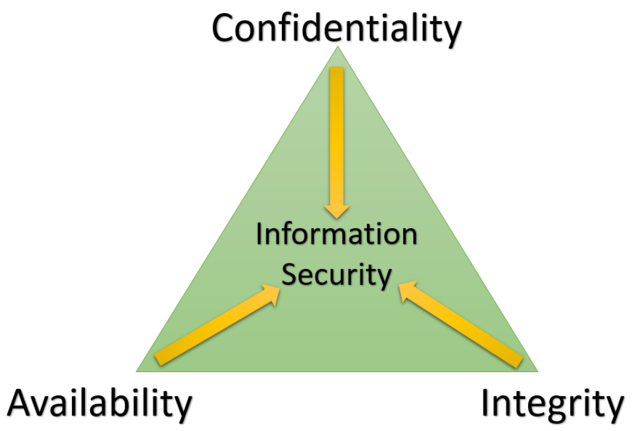
\includegraphics[scale=0.75]{Images/CIA_Triad}
\end{figure}
\end{frame}



\begin{frame}{Definitie}
\begin{itemize}
\item
Securitatea informaţiei este domeniul care se ocupă de \textbf{studiul mecanismelor de protecţie a informaţiei}, în scopul asigurării unui \textbf{nivel de încredere în informație}. 

\item
Nivelul de încredere în informaţie depinde de nivelul mecanismelor de securitate care îi garantează protecţia în fața riscurilor care apar asupra securităţii ei. 

\item
\textbf{Information Systems Security (INFOSEC)}*: \textbf{protecţia }sistemelor informatice împotriva:
\begin{itemize}
\item
\textbf{accesului neautorizat }
\item
sau a \textbf{modificării informaţiei}, fie stocată, procesată sau în tranzit, 
\item
şi \textbf{împotriva refuzului de servicii} către utilizatorii \textbf{autorizaţi }
\item
sau \textbf{asigurării de servicii }către utilizatorii \textbf{neautorizaţi}, 
\end{itemize}
incluzând acele metode necesare detectării, documentării şi respingerii acestor ameninţări.

* CNSS, (2006), NATIONAL INFORMATION ASSURANCE (IA) GLOSSARY
\end{itemize}
\end{frame}



\begin{frame}{Definiție}
\begin{itemize}
\item
Information Security requires for an information system \textbf{trust}.
\item
The system:
\begin{itemize}
\item
was designed properly
\item
was independently evaluated against a set of explicit security standards
\item
maintains proper operation during its lifetime, face of malicious attacks/human error
\end{itemize}
\end{itemize}
\end{frame}



\begin{frame}{Vulnerabilități}
\begin{itemize}
\item
Cum ajunge adversarul la sistemul informatic?
\begin{itemize}
\item
Securitatea fizica
\item
Securitatea electronică
\end{itemize}
\item
Information system’s vulnerabilities affect 3 levels of human activities:
\begin{itemize}
\item
personal security (privacy)
\item
companies/organization security
\item
national security
\end{itemize}
\end{itemize}
\end{frame}



\begin{frame}{Vulnerabilități}
\begin{itemize}
\item
In securitatea informației, cuvantul \textbf{vulnerabilitate} se refera la un punct slab in sistem care permite unui atacator să încalce unul sau mai multe dintre principiile/obiectivele acesteia.

\item
Regula: un sistem nu este mai sigur decât cea mai vulnerabilă componentă a sa.

\item
Clasificare vulnerabilitati:
\begin{itemize}
\item
\textbf{vulnerabilităţi de proiectare} (ex. proiectarea greşită a unui protocol de comunicare)
\item
\textbf{vulnerabilităţi de implementare} (ex. overflow) 
\item
\textbf{vulnerabilităţi de utilizare/exploatare} (ex. alegerea unor parole slabe, etc.)
\end{itemize}
\end{itemize}
\end{frame}



\begin{frame}{Vulnerabilități}
\begin{itemize}
\item
A vulnerability can exist either only in theory, or could have a known \textbf{exploit}. 
\item
Vulnerabilities are of significant interest when the program containing the vulnerability:
\begin{itemize}
\item
operates with special privileges,
\item
performs authentication,
\item
or provides easy access to user data or facilities (e.g. network server).
\end{itemize}
\end{itemize}
\end{frame}



\begin{frame}{Cauze ale vulnerabilităților}
\begin{itemize}
\item
vulnerabilitatea unei primitive criptografice ce poate fi amplificată de protocolul de securitate 
\begin{itemize}
\item
multe funcţii criptografice au vulnerabilităţi ascunse
\item
chiar şi folosirea celei mai solide funcţii criptografice în mod necorespunzător poate duce la pierderea totală a securităţii
\end{itemize}

\item
asumarea unor garanţii de securitate care sunt supra-specificate sau prost înţelese 
\begin{itemize}
\item
e.g. utilizarea unei funcţii de criptare şi prezumţia faptului că aceasta va asigura şi faptul că datele nu vor fi alterate
\end{itemize}

\item
neatenţia în aplicarea unor principii generale aplicabile unei clase mai largi de primitive 
\begin{itemize}
\item
e.g. criptarea folosind un mecanism cu cheie publică a unei informaţii de entropie scăzută
\end{itemize}
\end{itemize}
\end{frame}



\begin{frame}{Cauze ale vulnerabilităților}
\begin{itemize}
\item
lipsa definiţiilor formale

\item
lipsa unui buget de securitate incremental

\item
absenţa expertizei necesare în domeniul securităţii

\item
incapacitatea de a instala uşor tehnologia necesară

\item
politici de securitate inadecvate

\item
sisteme slabe de control ale reţelelor

\item
proasta configurare a sistemelor

\item
comunicare wireless neadecvată

\item
autentificare neadecvată la comunicare

\end{itemize}
\end{frame}



\begin{frame}{Cauze ale vulnerabilităților}
\begin{itemize}
\item
lipsa mecanismelor de detecţie şi restricţionare a drepturilor de acces la sisteme de control

\item
absenţa uneltelor pentru detecţia şi raportarea activităţilor anormale

\item
utilizarea reţelei pentru trafic neautorizat

\item
lipsa mecanismelor de detecţie a erorilor ce pot conduce la epuizarea bufferelor

\item
lipsa mecanismelor de control a schimbului de software

\item
lipsa educaţiei utilizatorilor cu privire la bunele practici în vederea asigurării securităţii

\end{itemize}
\end{frame}



\begin{frame}{Cauze ale vulnerabilităților}
\begin{itemize}
\item
Computer systems and programs have become \textbf{more complex}.

\item
\textbf{Quality control} hasn’t been able to keep up due to market pressures, programming skill deficiencies, etc. 
\begin{itemize}
\item
Quality control is a real issue when it comes to determining if a piece of code is “secure”. 
\item
Most companies simply don’t have the time to check ALL the possibilities because of a number of reasons
\item
e.g. Since there was no central UNIX development group, it was up to the individual programmers to check their code. 
\end{itemize}

\item
So Many Systems, Not Enough Time - 2.3 million hosts are connected to the Net each month.  

\item
\textbf{The Prime Directive: Keep the system up!}
\item
\textbf{Patch the system? When I will have time …}

\end{itemize}
\end{frame}



\begin{frame}{Disclosure of vulnerabilities}
\begin{itemize}
\item
The method of disclosing vulnerabilities is a topic of debate in the computer security community. 
\begin{itemize}
\item
Some advocate \textbf{immediate full disclosure} of information about vulnerabilities once they are discovered. 

\item
Others argue for \textbf{limiting disclosure} to the users placed at greatest risk, and only releasing full details after a delay, if ever. Such delays may allow those notified to fix the problem by developing and applying patches, but may also increase the risk to those not privy to full details. 
\end{itemize}

\item
This debate has a long history in security. 

\item
More recently a new form of commercial vulnerability disclosure has taken shape, see for example TippingPoint's Zero Day Initiative which provides a \textbf{legitimate market for the purchase and sale of vulnerability information }from the security community.

\end{itemize}
\end{frame}



\begin{frame}{Disclosure of vulnerabilities}
\begin{itemize}
\item
From the security perspective, only \textbf{a free and public disclosure} can ensure that all interested parties get the relevant information. 
\item
Security through obscurity is a concept that most experts consider unreliable.
\item
Most often a channel is considered trusted when it is a widely accepted source of security information in the industry (e.g. CERT, SecurityFocus, Secunia and FrSIRT). 

\end{itemize}
\end{frame}



\begin{frame}{Disclosure of vulnerabilities}
\begin{itemize}
\item
The \textbf{time of disclosure} of a vulnerability is defined differently in the security community and industry. It is most commonly referred to as "a kind of public disclosure of security information by a certain party". 

\item
The time of disclosure is the first date a security vulnerability is described on a channel where the disclosed information on the vulnerability has to fulfil the following requirement:
\begin{itemize}
\item
the information is freely available to the public 
\item
the vulnerability information is published by a trusted and independent channel/source 
\item
the vulnerability has undergone analysis by experts such that risk rating information is included upon disclosure 
\end{itemize}
\end{itemize}
\end{frame}



\begin{frame}{Vulnerabilități}
\begin{itemize}
\item
Many software \textbf{tools} exist that can aid in the discovery (and sometimes removal) of vulnerabilities in a computer system. 

\item
Though these tools can provide an auditor with a good overview of possible vulnerabilities present, \textbf{they can not replace human judgement}. Relying solely on scanners will yield false positives and a limited-scope view of the problems present in the system.

\item
Vulnerabilities have been found in \textbf{every major operating system}, including Windows, Mac OS, various forms of Unix and Linux, OpenVMS, and others. 

\end{itemize}
\end{frame}



\begin{frame}{Vulnerabilități}
\begin{itemize}
\item
The only way to reduce the chance of a vulnerability being used against a system is through \textbf{constant vigilance}:
\begin{itemize}
\item
\textbf{careful system maintenance} (e.g. applying software patches), 
\item
\textbf{best practices in deployment} (e.g. the use of firewalls and access controls) 
\item
and \textbf{auditing} (both during development and throughout the deployment lifecycle).
\end{itemize}
\end{itemize}
\end{frame}



\begin{frame}{Vulnerabilități}
\begin{itemize}
\item
Software tools
\begin{itemize}
\item
Altiris SecurityExpressions (Symantec)
\item
Citadel Security Software (McAfee)
\item
GFI LANguard (Network Security Scanner-GFI Software) 
\item
FusionVM  (Critical Watch) 
\item
QualysGuard (Qualys)
\item
Retina Network Security Scanner (Beyond Trust)
\item
STAT Guardian Vulnerability Management Suite (Harris Corporation)
\end{itemize}
\end{itemize}
\end{frame}



\begin{frame}{Amenințări}
\begin{itemize}
\item
Any good hacker can write the attack tool. 

\item
A small minority of hackers have the technical expertise to write some of the attack tools commonly in use.

\item
There are lots of hacker web sites where one can get these tools.

\item
These sites try to outdo each other by designing the best, baddest, user-friendly site. Sites like:
\begin{itemize}
\item
www.metasploit.com,
\item
www.insecure.org, 
\item
www.kali.org, 
\item
www.securityfocus.com 
\end{itemize}
 are examples of where one can download a wide variety of attacks tools. 
\item 
These sites \textbf{make it easy for anyone} who knows how to use a browser to get these tools. 

\end{itemize}
\end{frame}



\begin{frame}{Cine este adversarul?}
\begin{itemize}
\item
\textbf{Hackerii} dispun de resurse de calcul şi financiare scăzute şi atacă sisteme în general doar motivaţi de dorinţa de a brava sau pentru amuzament.

\item
\textbf{Clienţii unei reţele} au putere de calcul limitată şi sunt motivaţi de interese economice, de exemplu: fraudarea valorii facturate în reţeaua termo-electrică, etc.

\item
\textbf{Comercianţii} dispun de putere de calcul modestă şi de resurse financiare apreciabile având interes în aflarea sau manipularea secretelor pentru câştigarea avantajelor financiare.

\item
\textbf{Crima organizată} are putere de calcul modestă şi putere financiară ridicată având interes în alterarea parametrilor la care funcţionează sistemele pentru câştigarea unor avantaje financiare.
\end{itemize}
\end{frame}



\begin{frame}{Cine este adversarul?}
\begin{itemize}
\item
\textbf{Teroriştii} dispun de putere ridicată de calcul şi financiară fiind motivaţi de raţiuni politico-religioase cu scopul de a răspândii panică şi pagube de ordin financiar.

\item
\textbf{Guvernele} statelor adversare, dispun de putere de calcul şi financiară ridicată, şi mai mult, de operatori pricepuţi şi antrenaţi cu experienţă în domeniu. Scopul acestora este în general de a afecta infrastructurile în atacuri complexe de natură fizică sau electronică.

\item
\textbf{Oamenii din sistem} sunt persoane care deţin informaţii de detaliu şi au acces la elementele cheie în funcţionare, sunt motivaţi în general de interese sau nemulţumiri de ordin salarial/financiar.

\item
O combinaţie a variantelor de mai sus este cel mai periculos tip de adversar; în practică este posibilă orice combinaţie şi aceasta are cele mai mari şanse de succes într-un atac.

\end{itemize}
\end{frame}



\begin{frame}{Cine este adversarul?}
\begin{figure}[t]
\centering
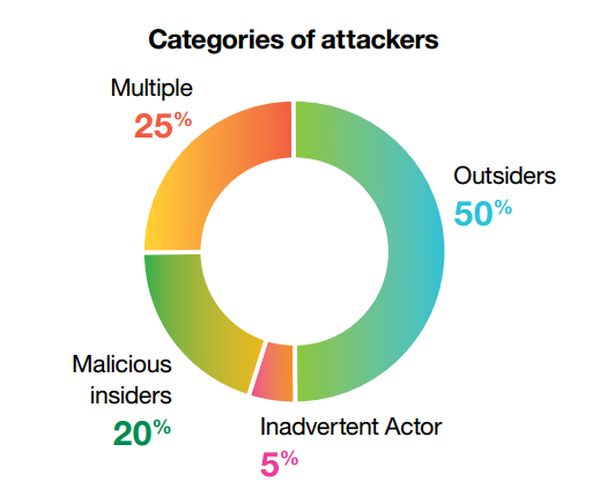
\includegraphics[scale=0.5]{Images/categories-of-attackers}
\caption{IBM Security Services Cyber Security Intelligence Index 2013}
\end{figure}
\end{frame}



\begin{frame}{Cine este adversarul?}
\begin{figure}[t]
\centering
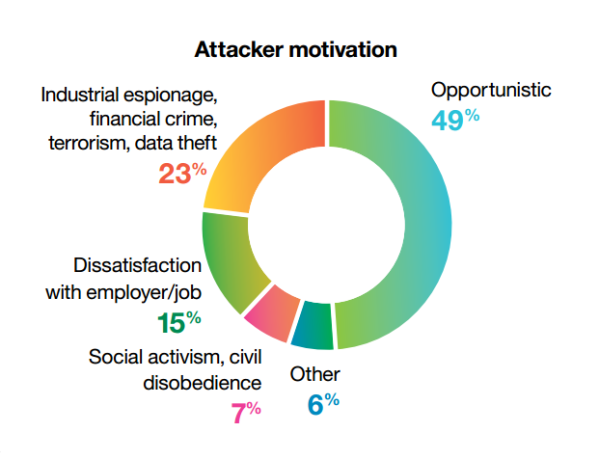
\includegraphics[scale=0.5]{Images/attacker-motivation}
\caption{IBM Security Services Cyber Security Intelligence Index 2013}
\end{figure}
\end{frame}



\begin{frame}{Amenințări}
177 Security Threats identified by ENISA (2016)
\begin{itemize}
\item
Identity theft (Identity Fraud/ Account)
\item
Denial of service
\item
Malicious code/ software/ activity
\item
Social Engineering
\item
Abuse of Information Leakage
\item
Manipulation of hardware and software
\item
Unauthorized installation of software
\item
Generation and use of rogue certificates (A false digital certificate used to secure Web sites)
\item
Compromising confidential information (data breaches)
\item
Remote activity (execution)
\item
Targeted attacks (APTs etc.)

...
\end{itemize}
\end{frame}



\begin{frame}{Amenințări}
\begin{itemize}
\item
\textbf{Malware} is software designed to infiltrate or damage a computer system without the owner's  consent. 
\begin{itemize}
\item
It is a blend of the words "malicious" and "software". 
\item
The expression means a variety of forms of hostile, intrusive, or annoying software or program code.
\end{itemize}

\item
\textbf{Spyware} is a type of program that watches what users do with their computer and then sends that information over the internet. 
\begin{itemize}
\item
Spyware can collect many different types of information about a user.
\item 
More benign programs can attempt to track what types of websites a user visits and send this information to an advertisement agency.
\item
More malicious versions can try to record what a user types to try to intercept passwords or credit card numbers. 
\item
Yet other versions simply launch popup advertisements.
\end{itemize}

\end{itemize}
\end{frame}



\begin{frame}{Amenințări}
\begin{itemize}
\item
\textbf{Adware} or advertising-supported software is any software package which automatically plays, displays, or downloads advertising material to a computer after the software is installed or while the application is being used.

\item
\textbf{Phishing} is a criminal activity using social engineering techniques. 
\begin{itemize}
\item
Phishers attempt to fraudulently acquire sensitive information, such as passwords and credit card details, by masquerading as a trustworthy person or business in an electronic communication.
\item
Phishing is typically carried out using email or an instant message, although phone contact has been used as well. 
\end{itemize}

\end{itemize}
\end{frame}



\begin{frame}{Amenințări}
\begin{itemize}
\item
\textbf{Ransomware} is a type of malicious software that threatens to publish the victim's data or perpetually block access to it unless a ransom is paid. 
\begin{itemize}
\item
some simple ransomware may lock the system in a way which is not difficult for a knowledgeable person to reverse
\item
more advanced malware uses a technique called cryptoviral extortion, in which it encrypts the victim's files, making them inaccessible, and demands a ransom payment to decrypt them
\end{itemize}
\end{itemize}
\end{frame}



\begin{frame}{Amenințări}
\begin{itemize}
\item
A \textbf{computer virus} is a type of malicious software that, when executed, replicates itself by modifying other computer programs and inserting its own code.
\begin{itemize}
\item
Viruses almost always corrupt or modify files on a targeted computer.
\end{itemize}

\item
A \textbf{computer worm} is a standalone malware computer program that replicates itself in order to spread to other computers.
\begin{itemize}
\item
Often, it uses a computer network to spread itself, relying on security failures on the target computer to access it. 
\item
Worms almost always cause at least some harm to the network, even if only by consuming bandwidth.
\end{itemize}
\end{itemize}
\end{frame}



\begin{frame}{Riscuri de securitate}
\begin{figure}[t]
\centering
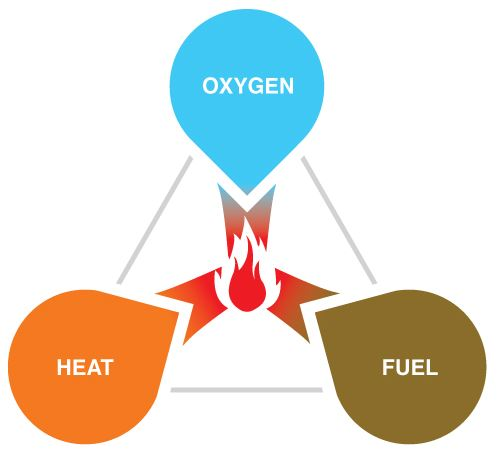
\includegraphics[scale=0.5]{Images/fire_triangle}
\end{figure}
\end{frame}



\begin{frame}{Riscuri de securitate}

\textbf{Atacator + Motivatie = Amenințare}

\textbf{Vulnerabilitate + Amenințare = Risc de securitate}

\begin{itemize}
\item
Concluzia de pana acum: există riscuri de securitate!

\item
Consecinţă a:
\begin{itemize}
\item
unor vulnerabilităţi în sistem
\item
a existenței unor potentiali adversari cu o anumită motivație
\end{itemize}

\item
Riscurile de securitate trebuie acoperite cu garanţii de securitate
\end{itemize}
\end{frame}



\begin{frame}{Riscuri de securitate}
\begin{figure}[t]
\centering
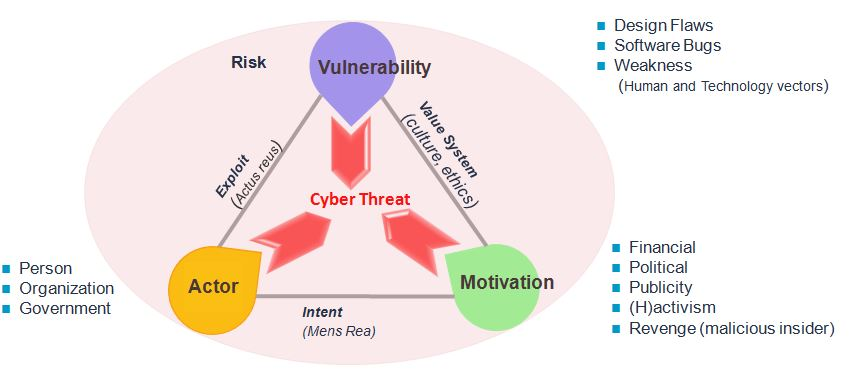
\includegraphics[scale=0.5]{Images/cybersecurity_triangle}
\end{figure}
\end{frame}



\begin{frame}{Atacuri cibernetice}
\begin{itemize}
\item
\textbf{Atac cibernetic} - agresiune asupra unui obiectiv de securitate

\item
Clasificare:

\begin{itemize}
\item
\textbf{atacuri pasive} 
\begin{itemize}
\item
modalitate: interceptare
\item
scop: citirea datelor, analiza de trafic, etc.
\end{itemize}

\item
\textbf{atacuri active} 
\begin{itemize}
\item
modalitate: întrerupere, modificare, fabricare
\item
scop: impersonare, replay, modificare, denial of service
\end{itemize}
\end{itemize}
\end{itemize}
\end{frame}



\begin{frame}{Atacuri pasive}
\begin{figure}[t]
\centering
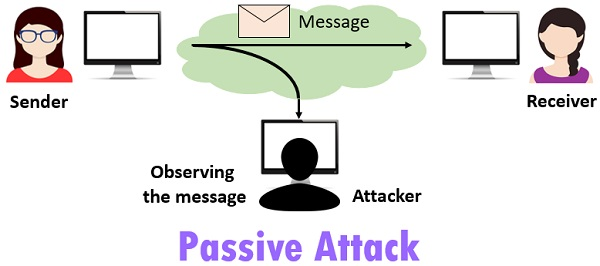
\includegraphics[scale=0.75]{Images/passive-attack-modified}
\end{figure}
\end{frame}



\begin{frame}{Atacuri active}
\begin{figure}[t]
\centering
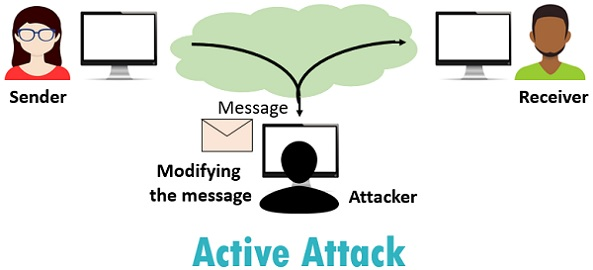
\includegraphics[scale=0.75]{Images/active-attack-modified}
\end{figure}
\end{frame}



\begin{frame}{Atacuri pasive versus Atacuri active}
\begin{figure}[t]
\centering
\begin{table}
\scalebox{0.75}{    
    \begin{tabularx}{\textwidth}{|X|X|X|}
    \hline
    \textbf{Basis for comparison}            & \textbf{Active Attack}                                                                 & \textbf{Passive Attack}                                                                                                   \\ \hline
    Basic                           & Active attack tries to change the system resources or affect their operation. & Passive attack tries to read or make use of information from the system but does not influence system resources. \\ \hline
    Modification in the information & Yes                                                                           & No                                                                                                               \\ \hline
    Harm to the system              & Yes                                                                           & No                                                                                                               \\ \hline
    Threat to                       & Integrity and availability                                                    & Confidentiality                                                                                                  \\ \hline
    Attack awareness                & The entity (victim) gets informed about the attack.                           & The entity is unaware of the attack.                                                                             \\ \hline
    Task performed by the attacker  & The transmission is captured by physically controlling the portion of a link. & Just need to observe the transmission.                                                                           \\ \hline
    Emphasis is on                  & Detection                                                                     & Prevention                                                                                                       \\ \hline
    \end{tabularx}}
\end{table}
\end{figure}
\end{frame}



\begin{frame}{Security Reports}
\begin{itemize}
\item
\textbf{Symantec 2018 Internet Security Threat Report}, vol. 23

\url{https://www.symantec.com/content/dam/symantec/docs/reports/istr-23-2018-en.pdf}

%\item
%\textbf{Symantec Executive Summary - 2018 Internet Security Threat Report}, vol. 23

%\url{https://www.symantec.com/content/dam/symantec/docs/reports/istr-23-executive-summary-en.pdf}

\item
\textbf{Akamai - State of the Internet Security Report}

\url{https://www.akamai.com/}

\url{https://www.akamai.com/us/en/about/our-thinking/state-of-the-internet-report/}

\item
\textbf{APWG Phishing Attack Trends Reports}

\url{https://www.antiphishing.org/}

\url{https://www.antiphishing.org/resources/apwg-reports/}

\end{itemize}
\end{frame}



\begin{frame}{Layers of security}
\begin{figure}[t]
\centering
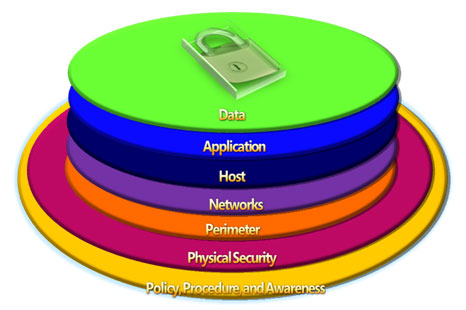
\includegraphics[scale=0.6]{Images/layers-of-security}
\end{figure}
\end{frame}



\begin{frame}{Layers of security}
\textbf{Data security}
\begin{itemize}
\item
concerns the protection of data from accidental or intentional but unauthorised modification, destruction or disclosure.

\begin{itemize}
\item
\textbf{Data Encryption} - converting the data into a code that cannot be easily read without a key that unlocks it.
\begin{itemize}
\item
disk encryption software
\item
disk encryption hardware
\end{itemize}
\item
\textbf{Data Masking} – masking certain areas of data so personnel without the required authorisation cannot look at it.
\item
\textbf{Data Erasure} – ensuring that no longer used data is completely removed and cannot be recovered by unauthorised people.
\item
\textbf{Data Backup} – creating copies of data so it can be recovered if the original copy is lost.
\end{itemize}
\end{itemize}
\end{frame}



\begin{frame}{Layers of security}
\begin{itemize}
\item
the chief principle - to offer protection to a data user’s collections or sources of data
\item
General Data Protection Regulations (\textbf{GDPR}) being enforced by the EU on 25 May 2018
\end{itemize}
\end{frame}



\begin{frame}{Layers of security}
\textbf{Application security}
\begin{itemize}
\item
applications are links between the data and the user (or another application)
\item
\textbf{application security versus software security}

\end{itemize}
\end{frame}



\begin{frame}{Layers of security}
\textbf{Software security (pre-deployment) activities include:}
\begin{itemize}
\item
Secure software design
\item
Development of \textbf{secure coding} guidelines for developers to follow
\item
Development of \textbf{secure configuration procedures and standards} for the deployment phase
\item
\textbf{Secure coding} that follows established guidelines
\item
\textbf{Validation of user input} and implementation of a suitable encoding strategy
\end{itemize}
\end{frame}



\begin{frame}{Layers of security}
\textbf{Software security (pre-deployment) activities include:}
\begin{itemize}
\item
\textbf{User authentication}
\item
User \textbf{session management}
\item
Function level access control
\item
Use of strong cryptography to \textbf{secure data} at rest and in transit
\item
Validation of third-party components
\item
Arrest of any flaws in software design/architecture
\end{itemize}
\end{frame}



\begin{frame}{Layers of security}
\textbf{Application security (post-deployment) activities include:}
\begin{itemize}
\item
Post deployment \textbf{security tests}
\item
Capture of flaws in software environment configuration
\item
\textbf{Malicious code detection} (implemented by the developer to create backdoor, time bomb)
\item
\textbf{Patch/upgrade}
\item
\textbf{IP filtering}
\item
Lock down executables
\item
Monitoring of programs at runtime to enforce the software use policy
\end{itemize}
\end{frame}



\begin{frame}{Layers of security}
\textbf{Host security}

\textbf{Host Based Security Best Practices} - Department of Computer Science Computing Guide - Princeton University:

\begin{itemize}
\item
Install and configure a host based firewall

\item
Choose good passwords for any accounts on the system, and change any default or well known accounts on the machine

\item
Install and keep up with operating system patches and also hardware firmware patches

\item
Configure and continue to monitor logs on the device

\end{itemize}
\end{frame}



\begin{frame}{Layers of security}
\begin{itemize}
\item
Disable services and accounts which are not being used, or are no longer necessary

\item
Replace insecure services (such as telnet, rsh, or rlogin) with more secure alternatives such as SSH

\item
Restrict access to services which cannot be disabled where possible

\item
Make and test backups of the system in a consistent manner

\end{itemize}
\end{frame}



\begin{frame}{Layers of security}
\textbf{Network security}
\begin{itemize}
\item
consists of the policies and practices adopted to prevent and monitor unauthorized access, misuse, modification, or denial of a computer network and network-accessible resources
\begin{itemize}
\item
authentication
\item
firewalls
\item
antivirus and antimalware software
\item
intrusion detection systems (IDS) and intrusion prevention systems (IPS)
\item
virtual private networks (VPN)
\item
honeypots
\end{itemize}
\end{itemize}
\end{frame}



\begin{frame}{Layers of security}
\textbf{Physical security}
\begin{itemize}
\item
security measures that are designed to deny unauthorized access to facilities, equipment and resources and to protect personnel and property from damage or harm

\item
deter potential intruders (e.g. warning signs and perimeter markings)

\begin{itemize}
\item
Physical barriers - for external threats: fences, walls, and vehicle barriers

\item
Combination barriers - for internal threats of fire, smoke migration as well as sabotage

\item
Natural surveillance - architects seek to build spaces that are more open and visible to security personnel and authorized users, so that intruders/attackers are unable to perform unauthorized activity without being seen

\item
Security lighting - intruders are less likely to enter well-lit areas for fear of being seen

\end{itemize}

\end{itemize}
\end{frame}



\begin{frame}{Layers of security}
\begin{itemize}
\item
detect intrusions and monitor/record intruders (e.g. intruder alarms and CCTV systems)
\begin{itemize}
\item
Alarm systems and sensors

\item
Video surveillance

\item
Access control

\item
Security personnel

\end{itemize}


\item
trigger appropriate incident responses (e.g. by security guards and police)

\end{itemize}
\end{frame}



\begin{frame}{Policy, Procedure and Awareness}
\begin{itemize}
\item
Information security policy is a \textbf{set of policies }issued by an organization to \textbf{ensure that all information technology users} within the domain of the organization or its networks \textbf{comply with rules and guidelines related to the security of the information} stored digitally at any point in the network or within the organization's boundaries of authority. 

\item
Key Elements of an Information Security Policy (see references)

\end{itemize}
\end{frame}



\begin{frame}{Policy, Procedure and Awareness}
\begin{figure}[t]
\centering
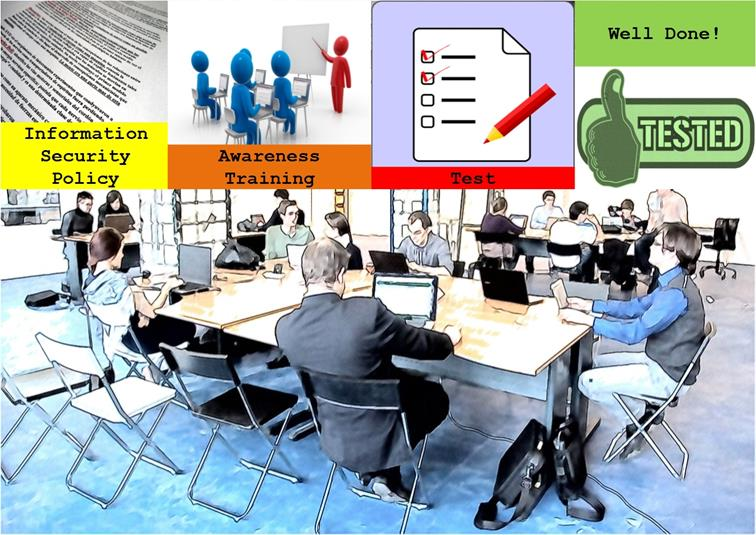
\includegraphics[scale=0.5]{Images/060614_1305_KeyElements12}
\end{figure}
\end{frame}



\begin{frame}{Policy, Procedure and Awareness}
\textbf{Key Elements of an Information Security Policy} (see references)
\begin{itemize}
\item
1 Purpose
\item
2 Scope
\item
3 Information security objectives
\item
4 Authority \& Access Control Policy
\item
5 Classification of Data
\item
6 Data Support \& Operations
\item
7 Security Awareness Sessions
\item
8 Responsibilities, Rights and Duties of Personnel
\item
9 Reference to Relevant Legislation
\item
10 Other Items
\end{itemize}
\end{frame}



\begin{frame}{Program licenta - Ingineria și securitatea sistemelor informatice militare - ATM}
Curriculum
\begin{itemize}
\item
Fundamente de securitate ciberneticǎ

\item
Securitatea sistemelor de operare

\item
Securitatea aplicaţiilor de baze de date

\item
Tehnici de analiza de cod maliţios

\item
Criptografie

\item
Testarea securității sistemelor informatice

\item
Managementul securității sistemelor informatice

\item
Sisteme biometrice

\end{itemize}
\end{frame}



\begin{frame}{Program master - Securitatea Tehnologiei Informației - ATM}
Curriculum
\begin{itemize}
\item
Matematici aplicate in ingineria securitatii informatiilor

\item
Criptografie computationala

\item
Semnaturi electronice si infrastructuri de securitate

\item
Protocoale de securitate

\item
Securitatea retelelor de calculatoare

\item
Securitatea sistemelor si aplicatiilor

\item
Securitatea bazelor de date

\item
Sisteme biometrice

\item
Securitatea multimedia

\item
Securitatea sistemelor electronice de plati

\end{itemize}
\end{frame}



\begin{frame}{Program master - Securitatea Tehnologiei Informației - ATM}
\begin{itemize}
\item
Reglementari privind securitatea cibernetica

\item
Strategii si politici de securitate cibernetica

\item
Razboi cibernetic

\item
Tehnologii pentru asigurarea continuitatii operationale

\item
Planificarea continuitatii operationale

\item
Evaluarea si managementul riscurilor

\item
Evaluarea si certificarea securitatii sistemelor

\item
Managementul securitatii informatiilor

\item
Criminalitatea informatica, colectarea si investigarea probelor

\end{itemize}
\end{frame}



\begin{frame}{Information Security Standards and Best Practices}
\begin{itemize}
\item
consist of a specific \textbf{set of rules, procedures or conventions} that are agreed upon between parties to perform business operations more uniformly and effectively

\item
can be viewed as a \textbf{set of predetermined guidelines} in
which the \textbf{issues, considerations and effects of doing something have already been analysed} by someone \textbf{authorised, experienced and qualified} in the specified area

\item
standards reflect industry best practices

\item
security and software development standards reflect industry best practices

\end{itemize}
\end{frame}



\begin{frame}{Information Security Standards and Best Practices}
\textbf{ISO/IEC 17799:2005 / ISO/IEC 27002:2007 / ISO/IEC 27002:2013}
\begin{itemize}
\item
ISO/IEC 27002:2013 — Information technology — Security techniques — Code of practice for information security controls (second edition) 

\item
provides best practice recommendations on information security controls for use by those responsible for initiating, implementing or maintaining information security management systems

\item
information security is defined within the standard in the context of the CIA triad

\item
objective: “\textbf{to ensure the selection of adequate and proportionate security controls that protect information assets and give confidence to interested parties including an organisation’s
customers}”

\end{itemize}
\end{frame}



\begin{frame}{Information Security Standards and Best Practices}
\textbf{ISO/IEC 17799:2005 / ISO/IEC 27002:2007 / ISO/IEC 27002:2013}
\begin{figure}[t]
\centering
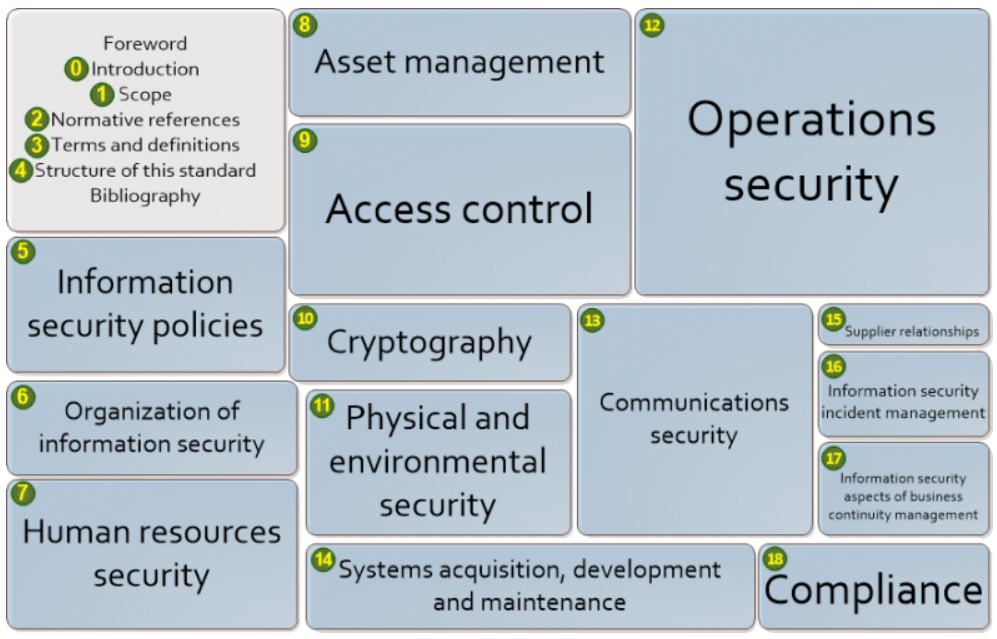
\includegraphics[scale=0.5]{Images/ISOIEC270022013}
\end{figure}
\end{frame}



\begin{frame}{Information Security Standards and Best Practices}
\textbf{ISO/IEC TR 13335 guideline}
\begin{itemize}
\item
guidelines for the management of IT security

\item
Part 1:
Concepts and Models

\item
Part 2:
Managing and Planning IT security

\item
Part 3:
Techniques for the Management of IT security – the complex topic of IT security risk assessment

\item
Part 4:
Selection of Safeguards

\item 
Part 5:
Safeguards for External Connections

\end{itemize}
\end{frame}



\begin{frame}{Information Security Standards and Best Practices}
\textbf{NIST security models}
\begin{itemize}
\item
\textbf{The NIST Cybersecurity Framework} (NIST CSF) "provides a high level taxonomy of cybersecurity outcomes and a methodology to assess and manage those outcomes." 

- It is intended to help private sector organizations that provide critical infrastructure with guidance on how to protect it, along with relevant protections for privacy and civil liberties.

\item
\textbf{Special publication 800-12} provides a broad overview of computer security and control areas. 

- It also emphasizes the importance of the security controls and ways to implement them. 

\item
\textbf{Special publication 800-14} describes common security principles that are used. 

- It provides a high level description of what should be incorporated within a computer security policy. 

- It describes what can be done to improve existing security as well as how to develop a new security practice. 

\end{itemize}
\end{frame}



\begin{frame}{Information Security Standards and Best Practices}
\begin{itemize}
\item
\textbf{Special publication 800-26} provides advice on how to manage IT security. Superseded by NIST SP 800-53 rev3. This document emphasizes the importance of self assessments as well as risk assessments.

\item
\textbf{Special publication 800-37} provides a new risk approach: "Guide for Applying the Risk Management Framework to Federal Information Systems".

\item
\textbf{Special publication 800-53} rev4, "Security and Privacy Controls for Federal Information Systems and Organizations", specifically addresses the 194 security controls that are applied to a system to make it "more secure".

\item
\textbf{Special Publication 800-82}, Revision 2, "Guide to Industrial Control System (ICS) Security" describes how to secure multiple types of Industrial Control Systems against cyber attacks while considering the performance, reliability and safety requirements specific to ICS. 
\end{itemize}
\end{frame}



\begin{frame}{Information Security Standards and Best Practices}
\textbf{Open systems security (interconnection standards)}
\begin{itemize}
\item
 ITU-T X.800 Recommendation: Security architecture for Open Systems Interconnection

\begin{itemize}
\item
a general description of security services and the related mechanisms that can be used to provide these services

\item
was developed specifically as the Open Systems Interconnection (OSI) security architecture, but the underlying concepts of X.800 have been shown to have much broader applicability 
\end{itemize}

\item
ITU-T X.805 Recommendation: Security architecture for systems providing end-to-end communications 

\end{itemize}
\end{frame}



\begin{frame}{Bibliography}
\textbf{Cărţi clasice despre Criptografie}
\begin{itemize}
\item
A.J. Menezes, P.C. Oorschot, S.A. Vanstone, (1996), Handbook of Applied Cryptography, CRC Press, 816 pagini, ISBN 0849385237.
\item
D. R. Stinson, (2005), Cryptography: Theory and Practice, Hall/CRC, 616 pagini, ISBN 1584885084.
\item
B. Schneier, (1996), Applied Cryptography, John Wiley \& Sons, 784 pagini, ISBN 0471117099.
\item
N. Ferguson (2003), B. Schneier, Practical Cryptography, Wiley

\end{itemize}
\end{frame}



\begin{frame}{Bibliography}

\textbf{Cărţi moderne despre Criptografie}
\begin{itemize}
\item
W. Mao, (2003), Modern Cryptography: Theory and Practice, Prentice Hall, 740 pagini, ISBN 0130669431.
\item
Jonathan Katz, Yehuda Lindell, (2007), Introduction to Modern Cryptography: Principles and Protocols, Hall/CRC Cryptography and Network Security Series, ISBN-10: 1584885513, ISBN-13: 978-1584885511.
\end{itemize}

\textbf{Cărţi despre Teoria Numerelor}
\begin{itemize}
\item
V. Shoup, (2004), Computational Introduction to Number Theory and Algebra
\end{itemize}

\end{frame}



\begin{frame}{Bibliography}
\textbf{Cărţi despre Securitatea informaţiei}
\begin{itemize}
\item
R. J. Anderson, (2001), Security Engineering: A Guide to Building Dependable Distributed Systems, Wiley, 640 pagini, ISBN 0471389226.
\item
W. Stallings, (2005), Cryptography and Network Security (4th Edition), Prentice Hall, 592 pagini, ISBN 0131873164.
\item
M.Togan, I. Florea, Infrastructuri de Securitate pentru Servicii Electronice în Internet, Ed. Matrix-Rom, 2017
\end{itemize}
\end{frame}



\begin{frame}{Bibliography}
\textbf{Articole științifice în cadrul conferințelor de specialitate}
\begin{itemize}
\item
Crypto \url{https://crypto.iacr.org/2018/}
\item
Eurocrypt \url{https://eurocrypt.iacr.org/2019/}
\item
Asiacrypt \url{https://asiacrypt.iacr.org/2018/}
\item
International Conference on Practice and Theory of Public Key Cryptography (PKC) \url{https://pkc.iacr.org/2018/}
\item
Fast Software Encryption (FSE) \url{https://fse.iacr.org/2018/}
\item
Theory of Cryptography (TCC) \url{https://tcc.iacr.org/2018/}
\item
Cryptographic Hardware and Embedded Systems (CHES) \url{https://ches.iacr.org/2018/}
\item
Real World Crypto Symposium (RWC) \url{https://rwc.iacr.org/}
\item
International Association for Cryptologic Research (IACR) - since 1982
\end{itemize}
\end{frame}



\begin{frame}{Bibliography}
\textbf{Digital Libraries, search engines, indexing services (some are free)}
\begin{itemize}
\item
Google Scholar \url{https://scholar.google.ro/}
\item
Microsoft Academic Search \url{https://academic.microsoft.com/}
\item
CiteSeerX \url{http://citeseerx.ist.psu.edu}
\item
Springer \url{https://www.springer.com/}
\item
IEEE Xplore Digital Library \url{https://ieeexplore.ieee.org/}
\item
SCI-HUB \url{https://sci-hub.tw/}
\item
etc.
\end{itemize}
\end{frame}



\begin{frame}{Bibliography}
\textbf{Search for the content of an article using SCI-HUB}
\begin{figure}[t]
\centering
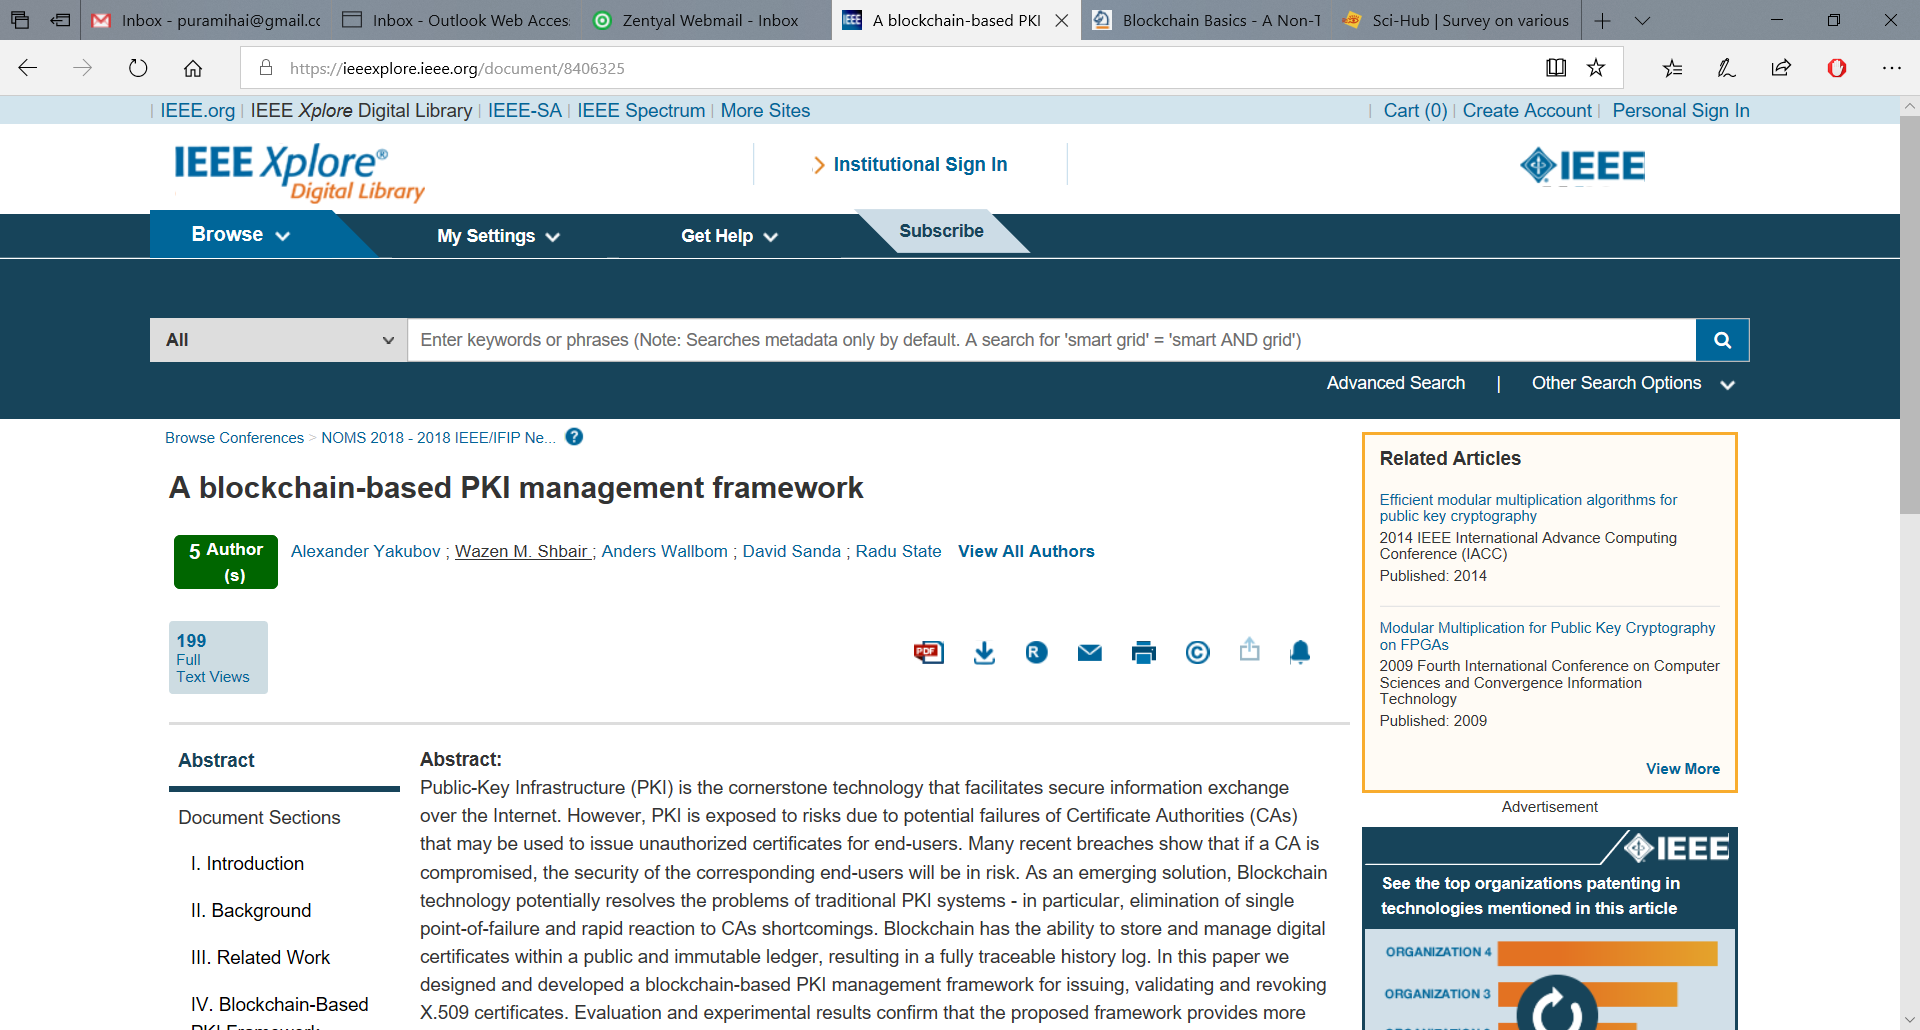
\includegraphics[scale=0.3]{Images/a}
\end{figure}
\end{frame}



\begin{frame}{Bibliography}
\textbf{Search for the content of an article using SCI-HUB}
\begin{figure}[t]
\centering
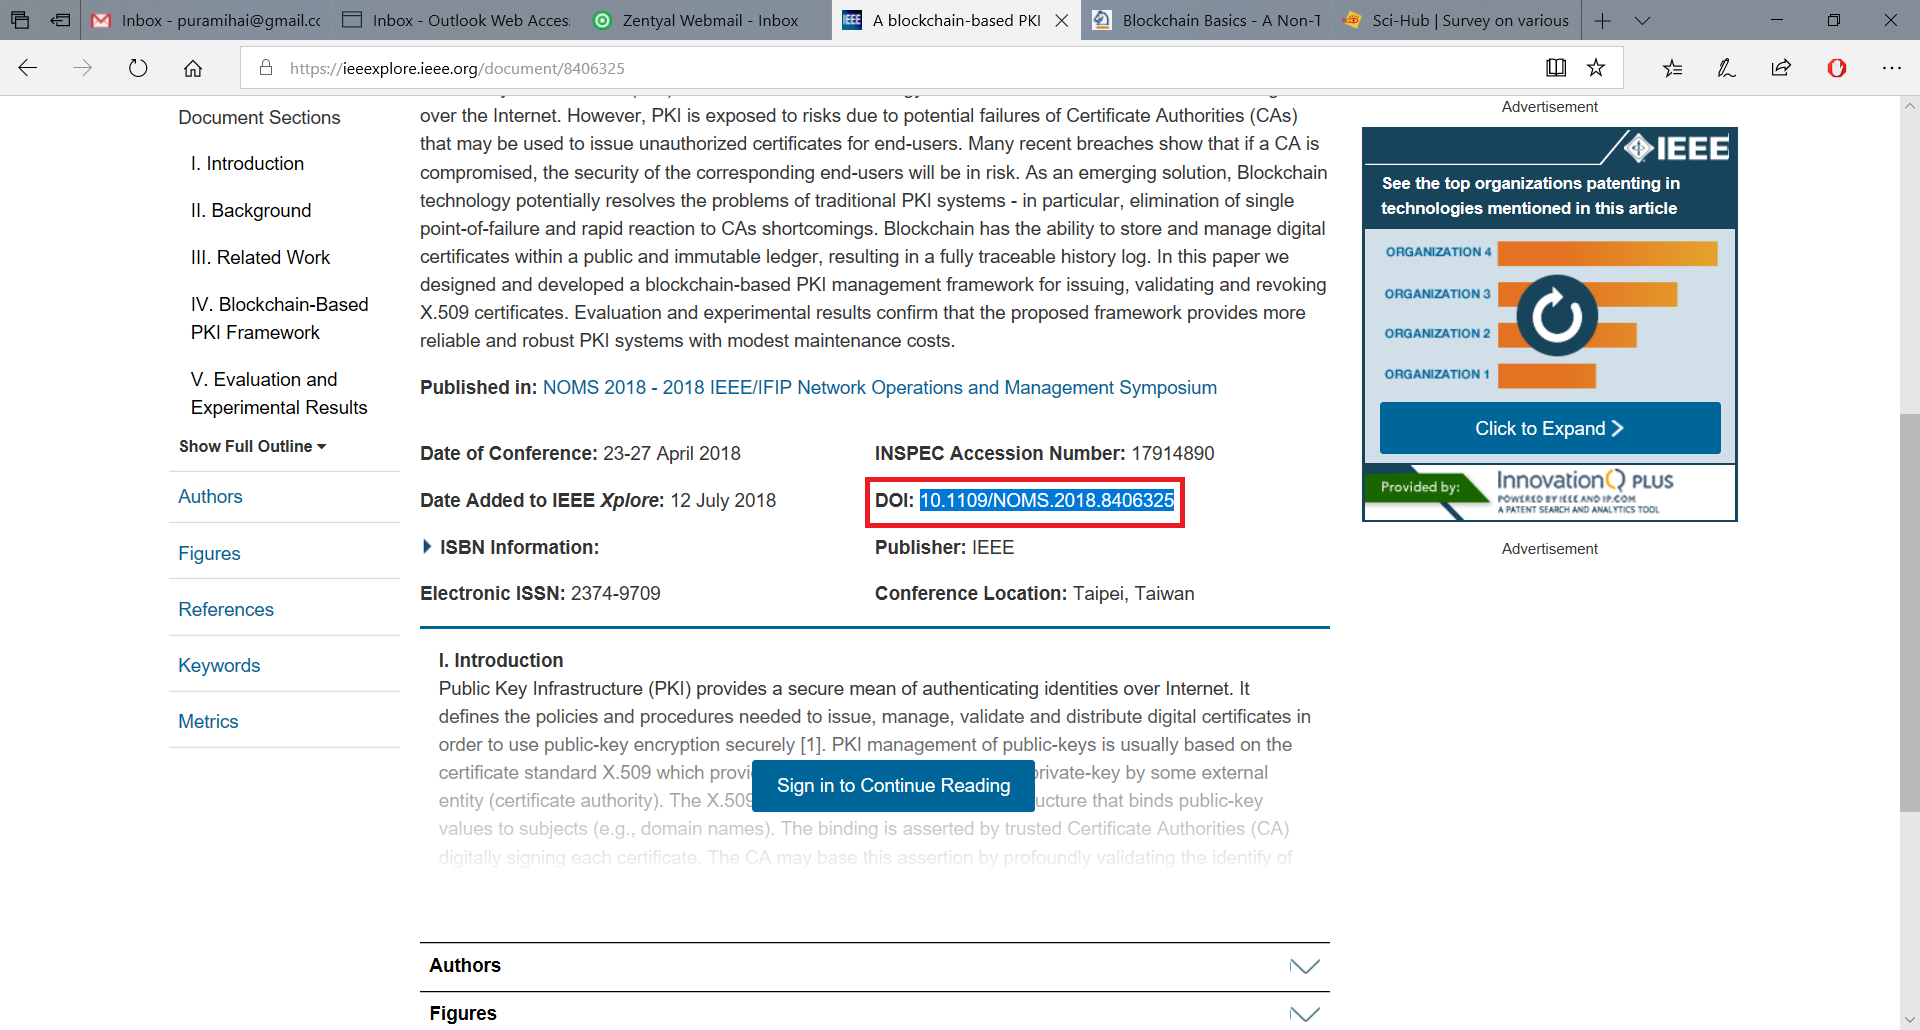
\includegraphics[scale=0.3]{Images/b}
\end{figure}
\end{frame}



\begin{frame}{Bibliography}
\textbf{Search for the content of an article using SCI-HUB}
\begin{figure}[t]
\centering
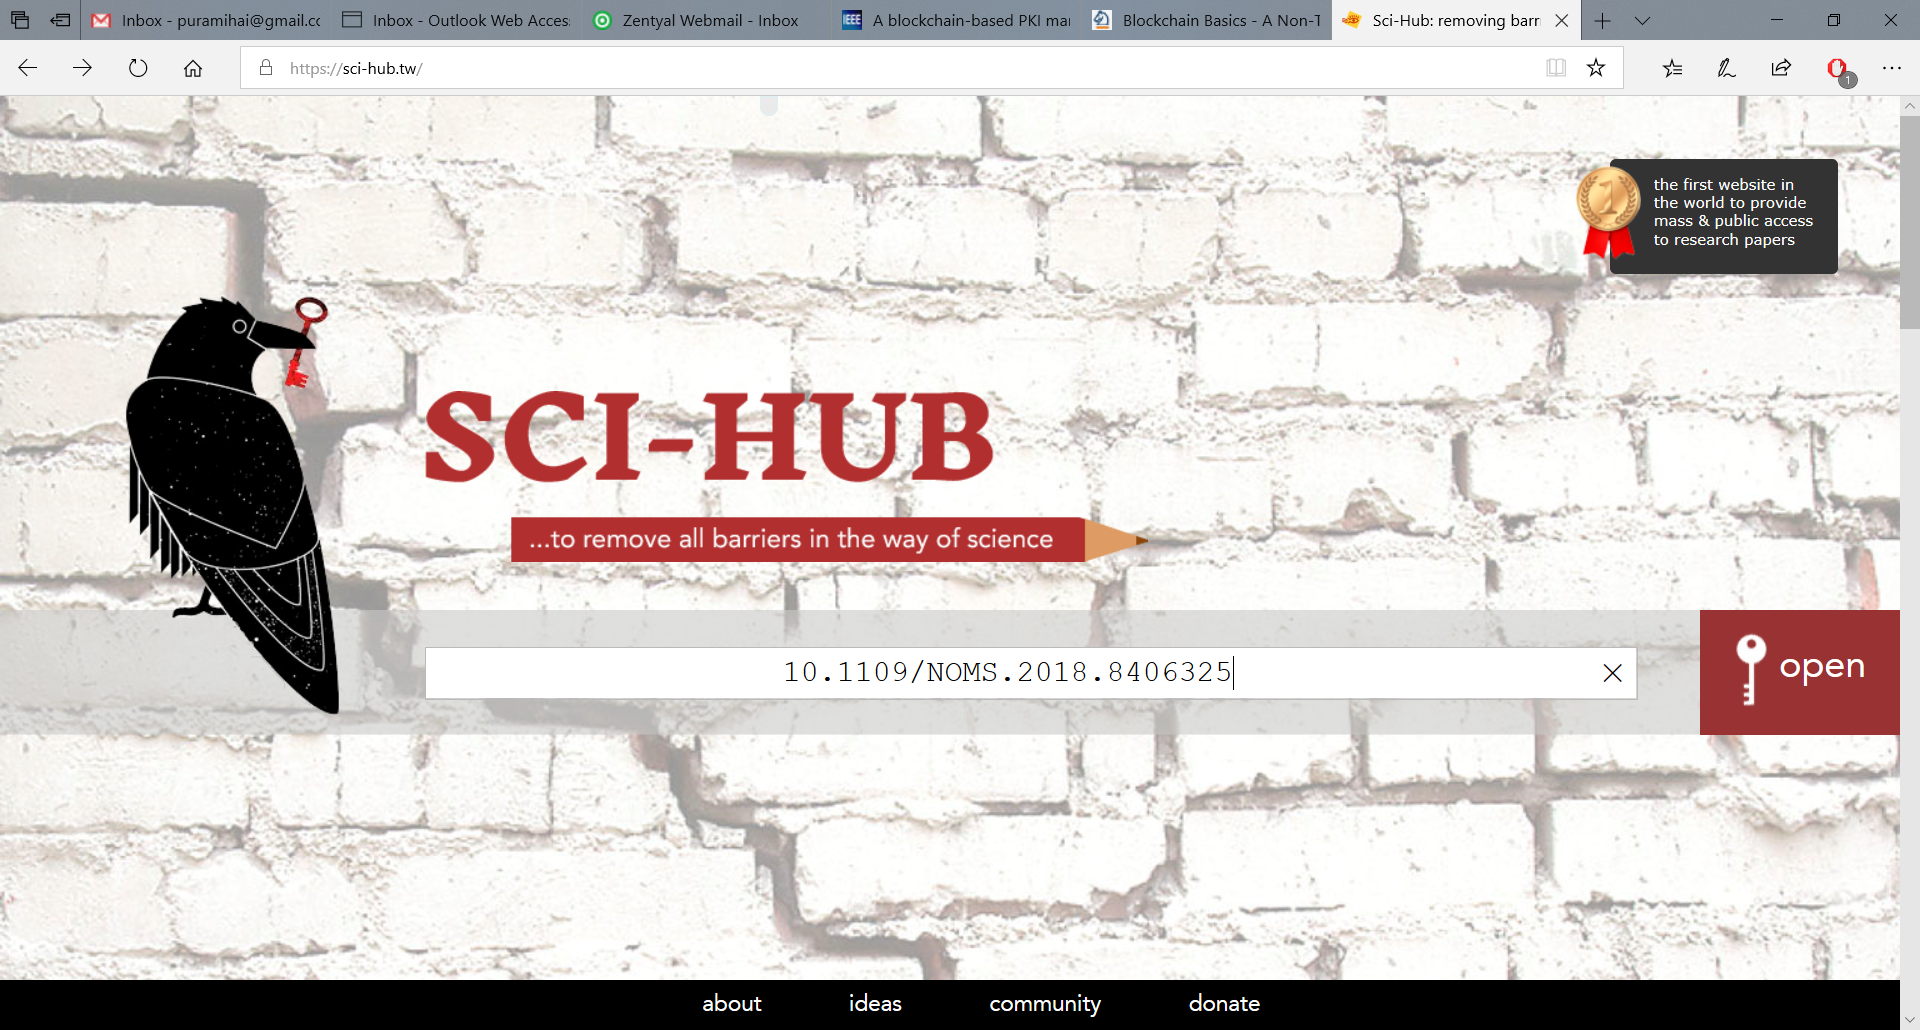
\includegraphics[scale=0.3]{Images/c}
\end{figure}
\end{frame}



\begin{frame}{Bibliography}
\textbf{Search for the content of an article using SCI-HUB}
\begin{figure}[t]
\centering
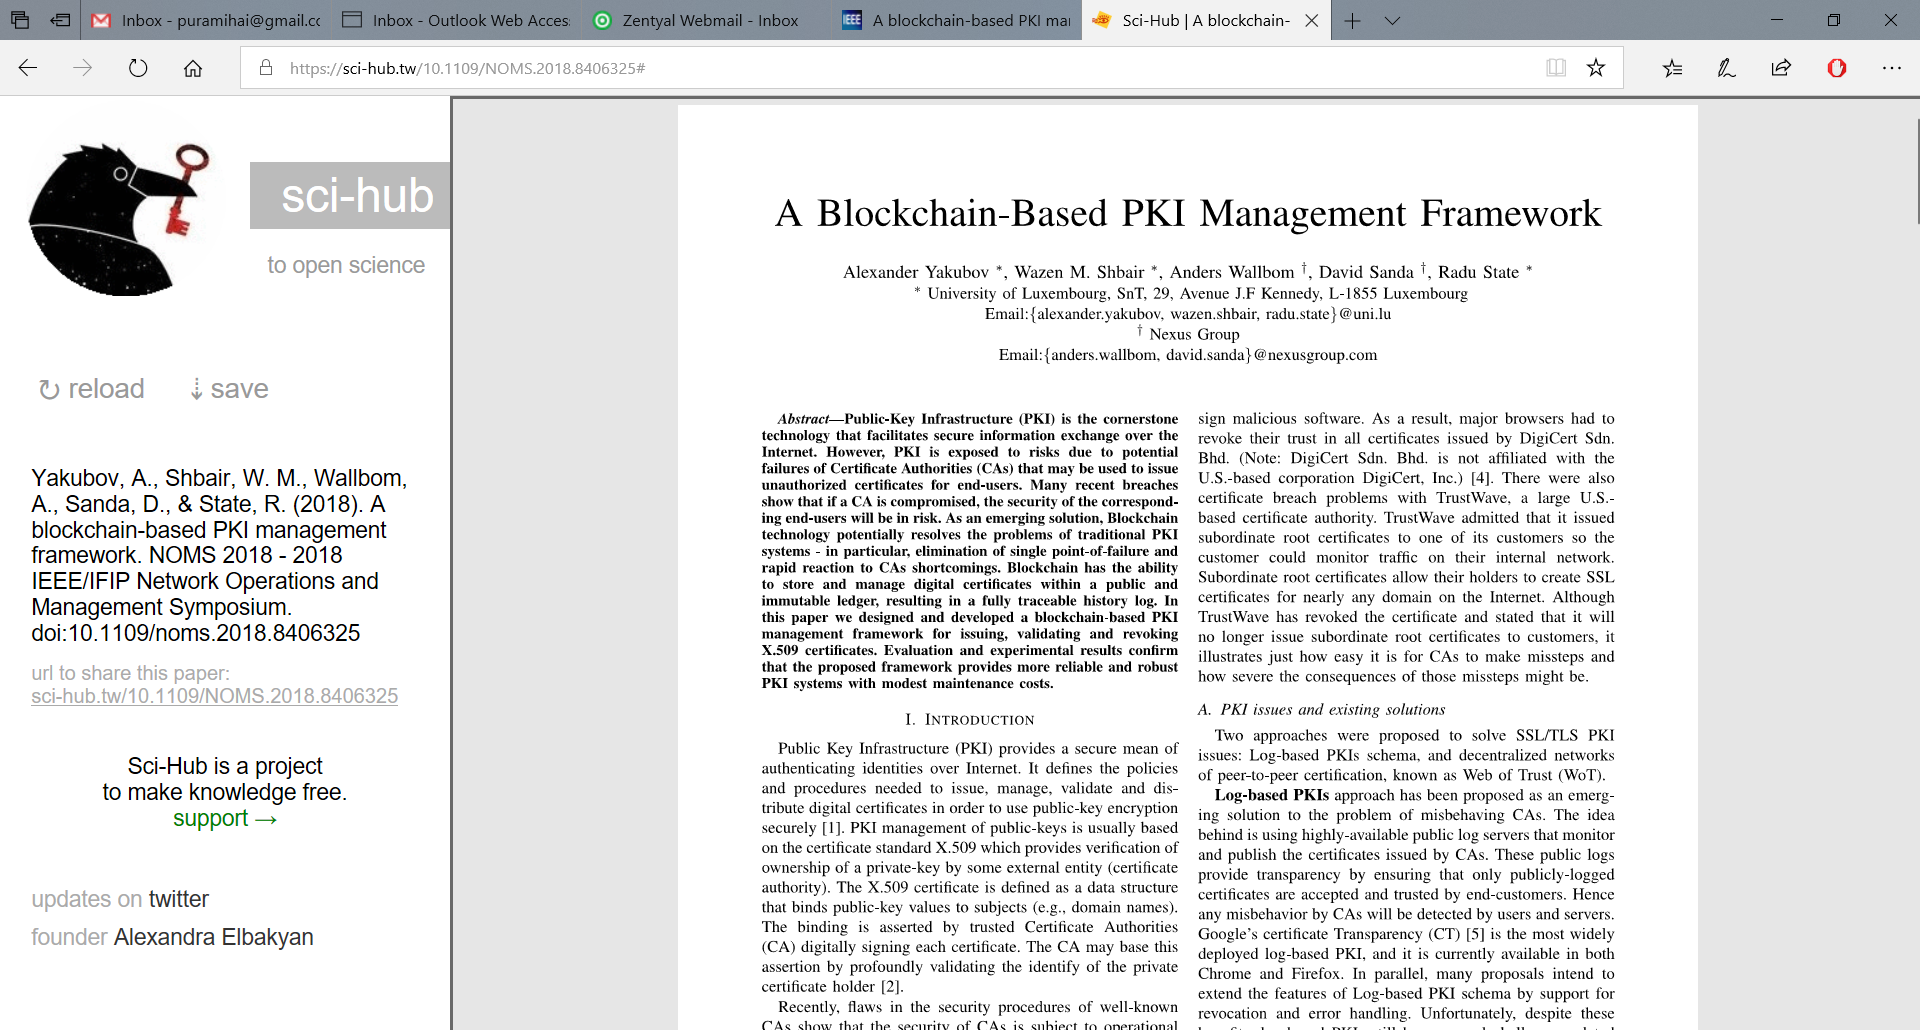
\includegraphics[scale=0.3]{Images/d}
\end{figure}
\end{frame}



\begin{frame}{Epilogue}

\begin{center}
\textbf{Security is a process, not a product.}
\end{center}

Bruce Schneier, prefață la lucrarea Secrets and Lies

\end{frame}



\begin{frame}{References}
\begin{itemize}
\item
Riham Yassin et al., Information Security

\url{https://www.slideshare.net/ahmedmoussaa/information-security-8332632}

\item
Lynn Ann Futcher, A Model for Integrating Information Security into the Software Development Life Cycle, MD Thesis, Nelson Mandela Metropolitan University, 2007

\url{https://www.academia.edu/745826/A_Model_for_Integrating_Information_Security_into_the_Software_Development_Life_Cycle}

\item
ENISA Threat Taxonomy - A tool for structuring threat information, 2016 

\url{https://www.enisa.europa.eu/topics/threat-risk-management/threats-and-trends/enisa-threat-landscape/etl2015/enisa-threat-taxonomy-a-tool-for-structuring-threat-information}
\end{itemize}
\end{frame}



\begin{frame}{References}
\begin{itemize}
\item
Illusion of CyberSecurity Part 2

\url{https://www.capgemini.com/2015/03/illusion-of-cybersecurity-part-2/}

\item
Andra Zaharia, Corporate Security Checklist – a CEO’s Guide to Cyber Security

\url{https://heimdalsecurity.com/blog/corporate-security-checklist-a-ceos-guide-to-cyber-security/}

\item
Difference Between Active and Passive Attacks

\url{https://techdifferences.com/difference-between-active-and-passive-attacks.html}

\item
Host Based Security Best Practices - Department of Computer Science Computing Guide - Princeton University:

\url{https://csguide.cs.princeton.edu/security/host}

\end{itemize}
\end{frame}



\begin{frame}{References}
\begin{itemize}
\item
Monika Chakraborty, Application security vs. software security: What’s the difference?

\url{https://www.synopsys.com/blogs/software-security/application-security-vs-software-security/}

\item
Key Elements of an Information Security Policy

\url{https://resources.infosecinstitute.com/key-elements-information-security-policy/}

\item
ISO/IEC 27002:2013 — Information technology — Security techniques — Code of practice for information security controls (second edition) 

\url{http://www.iso27001security.com/html/27002.html}

\item
Wikipedia
\end{itemize}
\end{frame}



\end{document}